\documentclass{standalone}
\usepackage{tikz}
\usetikzlibrary{patterns, positioning}
\usepackage[sfdefault]{ClearSans} %% option 'sfdefault' activates Clear Sans as the default text font
\usepackage[T1]{fontenc}

\begin{document}
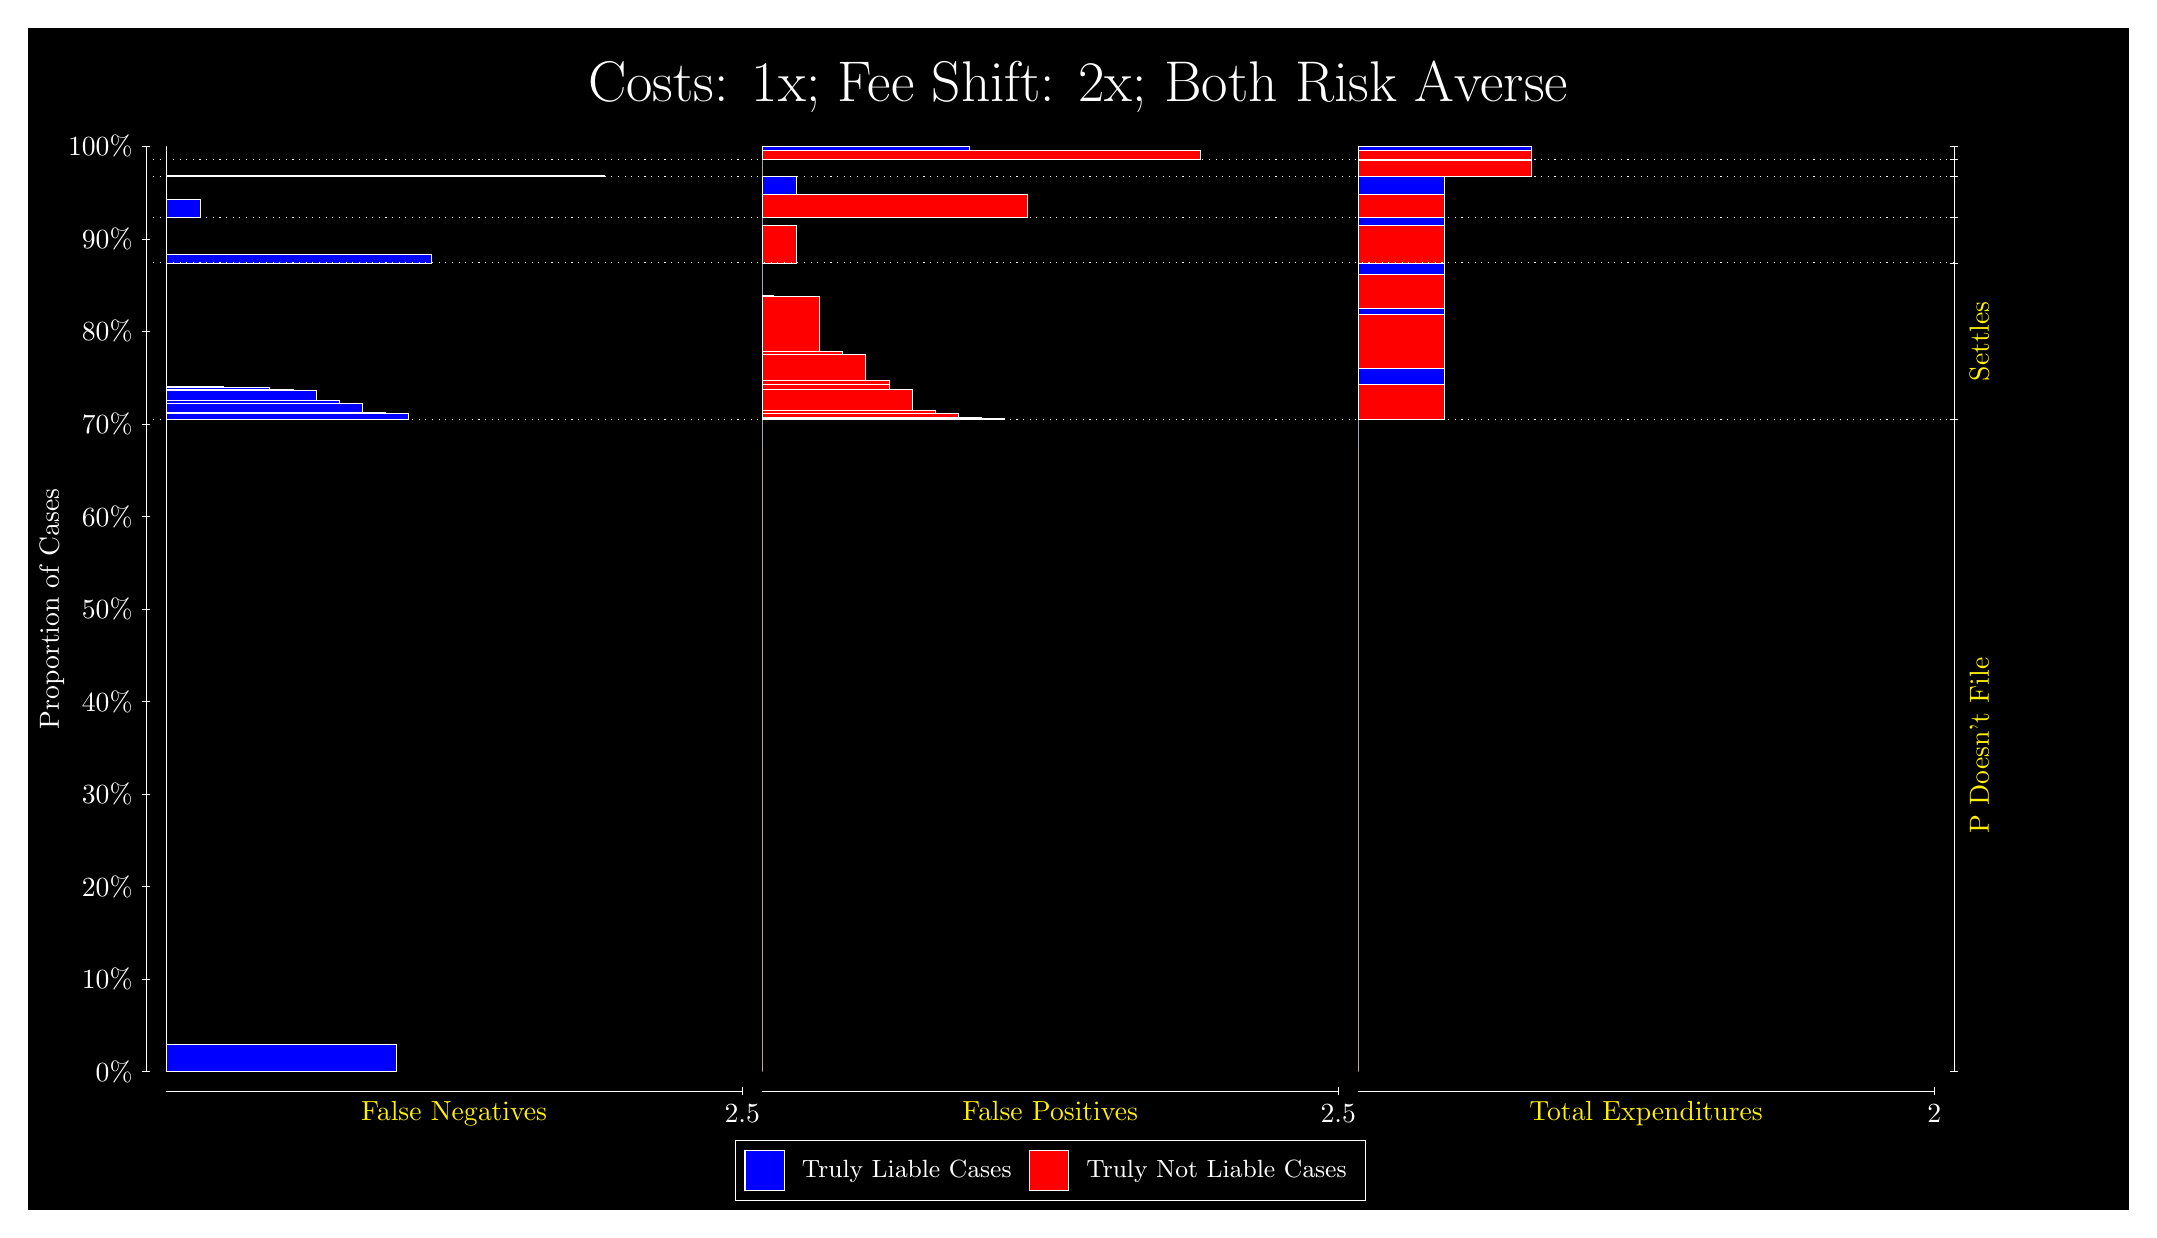
\begin{tikzpicture}
\draw[fill=black] (0,0) rectangle (26.667,15);
\draw[text=white] (0,13.5) rectangle (26.667,15) node[midway] {\huge Costs: 1x; Fee Shift: 2x; Both Risk Averse};
\draw[white, very thin] (1.5,1.75) -- (1.5,13.5);
\node[rotate=90, text=white, anchor=center] at (0.3, 7.625) {Proportion of Cases};
\draw[white, very thin] (1.45,1.75) -- (1.55,1.75);
\node[text=white, anchor=east] at (1.45, 1.75) {0\%};
\draw[white, very thin] (1.45,2.925) -- (1.55,2.925);
\node[text=white, anchor=east] at (1.45, 2.925) {10\%};
\draw[white, very thin] (1.45,4.1) -- (1.55,4.1);
\node[text=white, anchor=east] at (1.45, 4.1) {20\%};
\draw[white, very thin] (1.45,5.275) -- (1.55,5.275);
\node[text=white, anchor=east] at (1.45, 5.275) {30\%};
\draw[white, very thin] (1.45,6.45) -- (1.55,6.45);
\node[text=white, anchor=east] at (1.45, 6.45) {40\%};
\draw[white, very thin] (1.45,7.625) -- (1.55,7.625);
\node[text=white, anchor=east] at (1.45, 7.625) {50\%};
\draw[white, very thin] (1.45,8.8) -- (1.55,8.8);
\node[text=white, anchor=east] at (1.45, 8.8) {60\%};
\draw[white, very thin] (1.45,9.975) -- (1.55,9.975);
\node[text=white, anchor=east] at (1.45, 9.975) {70\%};
\draw[white, very thin] (1.45,11.15) -- (1.55,11.15);
\node[text=white, anchor=east] at (1.45, 11.15) {80\%};
\draw[white, very thin] (1.45,12.325) -- (1.55,12.325);
\node[text=white, anchor=east] at (1.45, 12.325) {90\%};
\draw[white, very thin] (1.45,13.5) -- (1.55,13.5);
\node[text=white, anchor=east] at (1.45, 13.5) {100\%};

\draw[white, very thin] (24.457,1.75) -- (24.457,13.5);
\draw[white, very thin] (24.407,1.75) -- (24.507,1.75);
\node[anchor=west] at (24.407, 1.75) {};
\draw[white, very thin] (24.407,10.03) -- (24.507,10.03);
\node[anchor=west] at (24.407, 10.03) {};
\draw[white, very thin] (24.407,12.019) -- (24.507,12.019);
\node[anchor=west] at (24.407, 12.019) {};
\draw[white, very thin] (24.407,12.598) -- (24.507,12.598);
\node[anchor=west] at (24.407, 12.598) {};
\draw[white, very thin] (24.407,13.119) -- (24.507,13.119);
\node[anchor=west] at (24.407, 13.119) {};
\draw[white, very thin] (24.407,13.335) -- (24.507,13.335);
\node[anchor=west] at (24.407, 13.335) {};
\draw[white, very thin] (24.407,13.5) -- (24.507,13.5);
\node[anchor=west] at (24.407, 13.5) {};

\draw[white, very thin, fill=blue] (1.75,1.75) rectangle (4.6775,2.0979);
\draw[white, very thin, fill=red] (1.75,2.0979) rectangle (1.75,10.03);
\draw[white, very thin, fill=blue] (1.75,10.03) rectangle (4.8239,10.107);
\draw[white, very thin, fill=blue] (1.75,10.107) rectangle (4.5312,10.121);
\draw[white, very thin, fill=blue] (1.75,10.121) rectangle (4.2384,10.237);
\draw[white, very thin, fill=blue] (1.75,10.237) rectangle (3.9457,10.281);
\draw[white, very thin, fill=blue] (1.75,10.281) rectangle (3.6529,10.396);
\draw[white, very thin, fill=blue] (1.75,10.396) rectangle (3.3602,10.416);
\draw[white, very thin, fill=blue] (1.75,10.416) rectangle (3.0674,10.437);
\draw[white, very thin, fill=blue] (1.75,10.437) rectangle (2.7746,10.443);
\draw[white, very thin, fill=blue] (1.75,10.443) rectangle (2.4819,10.455);
\draw[white, very thin, fill=red] (1.75,10.455) rectangle (1.75,12.019);
\draw[white, very thin, fill=blue] (1.75,12.019) rectangle (5.1167,12.125);
\draw[white, very thin, fill=red] (1.75,12.125) rectangle (1.75,12.598);
\draw[white, very thin, fill=blue] (1.75,12.598) rectangle (2.1891,12.825);
\draw[white, very thin, fill=red] (1.75,12.825) rectangle (1.75,13.119);
\draw[white, very thin, fill=blue] (1.75,13.119) rectangle (7.3123,13.131);
\draw[white, very thin, fill=red] (1.75,13.131) rectangle (1.75,13.335);
\draw[white, very thin, fill=red] (1.75,13.335) rectangle (1.75,13.445);
\draw[white, very thin, fill=blue] (1.75,13.445) rectangle (1.75,13.5);
\draw[white, very thin, fill=red] (9.3189,1.75) rectangle (9.3189,9.6821);
\draw[white, very thin, fill=blue] (9.3189,9.6821) rectangle (9.3189,10.03);
\draw[white, very thin, fill=red] (9.3189,10.03) rectangle (12.393,10.049);
\draw[white, very thin, fill=red] (9.3189,10.049) rectangle (12.1,10.061);
\draw[white, very thin, fill=red] (9.3189,10.061) rectangle (11.807,10.105);
\draw[white, very thin, fill=red] (9.3189,10.105) rectangle (11.515,10.149);
\draw[white, very thin, fill=red] (9.3189,10.149) rectangle (11.222,10.414);
\draw[white, very thin, fill=red] (9.3189,10.414) rectangle (10.929,10.477);
\draw[white, very thin, fill=red] (9.3189,10.477) rectangle (10.929,10.529);
\draw[white, very thin, fill=red] (9.3189,10.529) rectangle (10.636,10.857);
\draw[white, very thin, fill=red] (9.3189,10.857) rectangle (10.344,10.903);
\draw[white, very thin, fill=red] (9.3189,10.903) rectangle (10.051,11.593);
\draw[white, very thin, fill=blue] (9.3189,11.593) rectangle (9.4652,11.605);
\draw[white, very thin, fill=blue] (9.3189,11.605) rectangle (9.3189,12.019);
\draw[white, very thin, fill=red] (9.3189,12.019) rectangle (9.758,12.491);
\draw[white, very thin, fill=blue] (9.3189,12.491) rectangle (9.3189,12.598);
\draw[white, very thin, fill=red] (9.3189,12.598) rectangle (12.686,12.891);
\draw[white, very thin, fill=blue] (9.3189,12.891) rectangle (9.758,13.119);
\draw[white, very thin, fill=red] (9.3189,13.119) rectangle (9.3189,13.323);
\draw[white, very thin, fill=blue] (9.3189,13.323) rectangle (9.3189,13.335);
\draw[white, very thin, fill=red] (9.3189,13.335) rectangle (14.881,13.445);
\draw[white, very thin, fill=blue] (9.3189,13.445) rectangle (11.954,13.5);
\draw[white, very thin, fill=red] (16.888,1.75) rectangle (16.888,9.6821);
\draw[white, very thin, fill=blue] (16.888,9.6821) rectangle (16.888,10.03);
\draw[white, very thin, fill=red] (16.888,10.03) rectangle (17.986,10.477);
\draw[white, very thin, fill=blue] (16.888,10.477) rectangle (17.986,10.675);
\draw[white, very thin, fill=red] (16.888,10.675) rectangle (17.986,11.365);
\draw[white, very thin, fill=blue] (16.888,11.365) rectangle (17.986,11.442);
\draw[white, very thin, fill=red] (16.888,11.442) rectangle (17.986,11.869);
\draw[white, very thin, fill=blue] (16.888,11.869) rectangle (17.986,12.019);
\draw[white, very thin, fill=red] (16.888,12.019) rectangle (17.986,12.491);
\draw[white, very thin, fill=blue] (16.888,12.491) rectangle (17.986,12.598);
\draw[white, very thin, fill=red] (16.888,12.598) rectangle (17.986,12.891);
\draw[white, very thin, fill=blue] (16.888,12.891) rectangle (17.986,13.119);
\draw[white, very thin, fill=red] (16.888,13.119) rectangle (19.083,13.323);
\draw[white, very thin, fill=blue] (16.888,13.323) rectangle (19.083,13.335);
\draw[white, very thin, fill=red] (16.888,13.335) rectangle (19.083,13.445);
\draw[white, very thin, fill=blue] (16.888,13.445) rectangle (19.083,13.5);
\draw[white, dotted] (1.5,10.03) -- (24.457,10.03);
\draw[white, dotted] (1.5,12.019) -- (24.457,12.019);
\draw[white, dotted] (1.5,12.598) -- (24.457,12.598);
\draw[white, dotted] (1.5,13.119) -- (24.457,13.119);
\draw[white, dotted] (1.5,13.335) -- (24.457,13.335);
\draw[white, very thin] (1.75,1.5) -- (9.0689,1.5);
\node[text=yellow, anchor=north] at (5.4094, 1.5) {False Negatives};
\draw[white, very thin] (9.0689,1.45) -- (9.0689,1.55);
\node[text=white, anchor=north] at (9.0689, 1.45) {2.5};

\draw[white, very thin] (9.3189,1.5) -- (16.638,1.5);
\node[text=yellow, anchor=north] at (12.978, 1.5) {False Positives};
\draw[white, very thin] (16.638,1.45) -- (16.638,1.55);
\node[text=white, anchor=north] at (16.638, 1.45) {2.5};

\draw[white, very thin] (16.888,1.5) -- (24.207,1.5);
\node[text=yellow, anchor=north] at (20.547, 1.5) {Total Expenditures};
\draw[white, very thin] (24.207,1.45) -- (24.207,1.55);
\node[text=white, anchor=north] at (24.207, 1.45) {2};

\node[text=yellow, centered, rotate=90] at (24.777, 5.89) {P Doesn't File};
\node[text=yellow, centered, rotate=90] at (24.777, 11.024) {Settles};





\draw (12.978300999999998,1.5) node[draw=none] (baseCoordinate) {};
\begin{scope}[align=center]
        \matrix[scale=0.5, draw=white, below=0.5cm of baseCoordinate, nodes={draw}, column sep=0.1cm]{
            \node[rectangle, draw, minimum width=0.5cm, minimum height=0.5cm, fill=blue] {}; &
            \node[draw=none, font=\small, text=white] (B) {Truly Liable Cases}; &
            \node[rectangle, draw, minimum width=0.5cm, minimum height=0.5cm, fill=red] {}; &
            \node[draw=none, font=\small, text=white] (B) {Truly Not Liable Cases}; \\
            };
\end{scope}

\end{tikzpicture}
\end{document}